%% Q2D2 Quantization and Emergent Cross-Lingual Structure in a Low-Bitrate JEPA Speech Codec
%% Target venue: APSIPA ASC 2026 (4-6 pages, IEEE conference format, single-blind)
%% Compile: pdflatex main && bibtex main && pdflatex main && pdflatex main
%% All numbers traced to PAPER_CONTENT_MASTER.md (verified source-of-truth, 2026-05-14).
%% Inline flags: %% TODO and %% VERIFY mark items needing author action before submission.

\documentclass[conference,a4paper]{APSIPA2026}
\IEEEoverridecommandlockouts
\usepackage[a4paper, top=19mm, bottom=43mm, left=13mm, right=13mm]{geometry}
\usepackage{cite}
\usepackage{amsmath,amssymb,amsfonts}
\usepackage{algorithmic}
\usepackage{graphicx}
\usepackage{textcomp}
\usepackage{xcolor}
\usepackage{booktabs}
\usepackage{multirow}
\usepackage{float}
\usepackage{placeins}
\usepackage{fontawesome5}
\usepackage{url}
\usepackage[draft,bookmarks=false,pdfpagemode=UseNone]{hyperref}
% EDAS forbids PDF bookmarks (FAQ 115) and URL link annotations (FAQ 221).
% hyperref `draft` keeps \href{url}{text} rendering its visible TEXT but emits
% no link annotation; bookmarks=false suppresses the PDF outline.
\usepackage{fancyhdr}
\renewcommand{\headrulewidth}{0pt}
\renewcommand{\footrulewidth}{0pt}
\fancypagestyle{firststyle}{
  \fancyhf{}
  \fancyhead[C]{2026 Asia Pacific Signal and Information Processing Association Annual Summit and Conference (APSIPA ASC)}
}
\def\BibTeX{{\rm B\kern-.05em{\sc i\kern-.025em b}\kern-.08em
    T\kern-.1667em\lower.7ex\hbox{E}\kern-.125emX}}

\begin{document}

\title{JEPA-Q2D2: A Low-Bitrate Speech Codec\\
with Emergent Cross-Lingual Structure}

%% VERIFY author block before submission (APSIPA is single-blind, names ARE included)
\author{
\IEEEauthorblockN{Anant Shukla, Aman Anand, Suryansh Shakya, Vatsal Bharti
\thanks{All authors at rumik.ai. Correspondence: anant@rumik.ai.}}
\IEEEauthorblockA{\raisebox{-2pt}{
\includegraphics[height=11pt]{figures/rumik_logo.jpg}}\,\href{https://rumik.ai/}{\textit{rumik.ai}} \\
anant@rumik.ai \\[3pt]
{\small \faGithub\ \href{https://github.com/anant-004/jepa-q2d2}{github.com/anant-004/jepa-q2d2}}}
}

\maketitle
\thispagestyle{firststyle}
\pagestyle{empty}

\begin{abstract}
We present a $1.6$\,kbps neural speech codec that pairs a JEPA
(Joint-Embedding Predictive Architecture) encoder with Q2D2, a geometry-aware
two-dimensional lattice quantizer, and is trained without adversarial losses.
Q2D2 quantizes latent dimension pairs on a rhombic lattice with per-pair
learned affine transforms; a frozen WavLM perceptual loss is used during
decoder training. Under an identical internal ablation protocol, Q2D2 improves
over finite scalar quantization (FSQ) by $+0.37$ PESQ at a matched bitrate.
On a separate fixed $50$-utterance LibriLight evaluation, the codec reaches
PESQ\,$2.53$ and ESTOI\,$0.80$ at $1.6$\,kbps, exceeding EnCodec at a
comparable operating point but trailing Mimi on ESTOI. We further show that
SIGReg, a Gaussianizing regularizer applied to the Stage-1 encoder, prevents
Q2D2 collapse in a more aggressive $25$\,Hz / cd32 regime.
Despite English-only LibriLight training, the codec's pre-quantization encoder
features on held-out FLEURS speech (five unseen non-English languages plus a
disjoint English subset) reach $85.4\%$ $5$-NN language separability, higher
than every neural-codec baseline (Mimi, EnCodec, DAC) and every multilingual
SSL model we test (XLS-R-300m, mHuBERT-147), approaching uncompressed English
wav2vec2-base.
\end{abstract}

\begin{IEEEkeywords}
neural speech codec, vector quantization, lattice quantization,
self-supervised learning, cross-lingual representation
\end{IEEEkeywords}

\begin{figure*}[t]
\centering
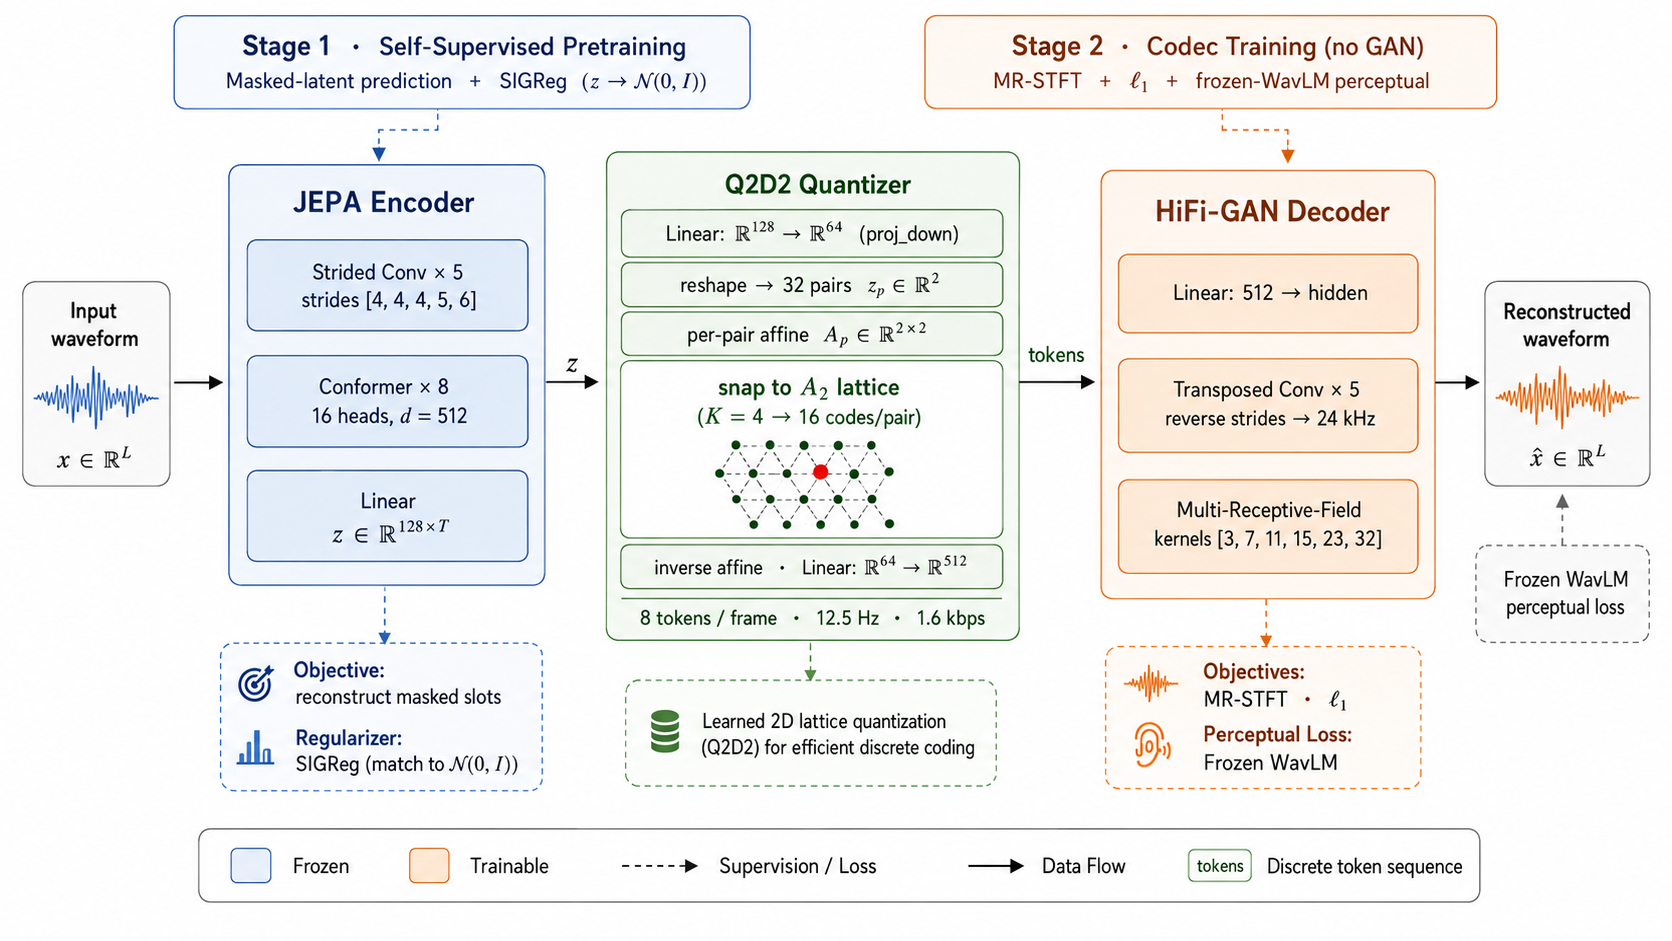
\includegraphics[width=0.95\textwidth]{figures/jepa_q2d2_architecture_2.png}
\caption{Codec architecture. A JEPA encoder maps the waveform to a
$128$-dimensional latent $z$; Q2D2 quantizes dimension pairs on a rhombic
lattice with per-pair learned affine transforms; a HiFi-GAN decoder reconstructs
audio. SIGReg shapes the encoder distribution during Stage~1; Stage~2 uses
multi-resolution STFT, $\ell_1$ and frozen-WavLM perceptual losses, with no GAN
discriminator.}
\label{fig:arch}
\end{figure*}

\section{Introduction}

\begin{figure}[t]
\centering
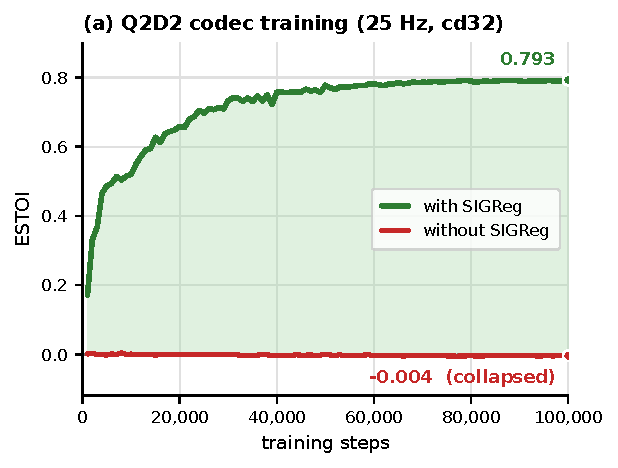
\includegraphics[width=\columnwidth]{figures/sigreg_panel_a.pdf}
\caption{SIGReg distribution-quantizer co-design. Two Q2D2 codecs at an
aggressive $25$\,Hz / $32$-dimensional operating point, identical except for
the SIGReg weight used to train the Stage~1 encoder. Without SIGReg
($\lambda_{\mathrm{sigreg}}{=}0$, red) the codec never leaves the floor; with
SIGReg ($\lambda_{\mathrm{sigreg}}{=}0.05$, green) the same codec trains
normally to ESTOI $0.79$. See Section~\ref{sec:sigreg}.}
\label{fig:sigreg}
\end{figure}

Discrete speech codecs have become the interface between waveforms and
language models: an autoregressive (AR) text-to-speech (TTS) system predicts
codec tokens, which a decoder renders to audio. This use case imposes two
demands that differ from classical speech coding. First, the token stream must
be \emph{short} (an AR model pays a quadratic cost in sequence length), so
the codec should operate at a low frame rate and a low bitrate. Second,
training must be \emph{stable and simple}, because codec quality directly
bounds downstream TTS quality and because practitioners increasingly train
many codec variants.

Most recent neural codecs \cite{encodec,dac,mimi,wavtokenizer} answer the
first demand with residual vector quantization (RVQ) and the second with
multi-scale GAN discriminators. Both choices have costs. RVQ and learned
vector quantization (VQ) are prone to codebook collapse and require commitment
losses and careful initialization. GAN discriminators introduce a non-stationary
adversarial objective whose instability is well documented. Finite scalar
quantization (FSQ) \cite{fsq} removes codebook learning but quantizes each
latent dimension independently on an axis-aligned grid, ignoring correlations
between dimensions.

We study a codec built from two components chosen to address these costs
directly. The encoder is a JEPA model \cite{jepa_tokenizer}, a self-supervised
architecture that predicts masked latent features rather than reconstructing
inputs; it is trained from scratch on English-only LibriLight. The quantizer
is Q2D2 \cite{q2d2}, which groups latent dimensions into pairs and snaps each
pair to a rhombic ($A_2$) lattice after a per-pair learned affine transform.
Because lattice quantization is provably efficient only for sources that match
the lattice geometry, we additionally shape the encoder distribution with
SIGReg, a Cram\'er--Wold Gaussianizing regularizer, and we train the decoder
with a frozen-WavLM perceptual loss and no adversarial losses.

The main contributions of this paper are:

\begin{enumerate}
\item \textbf{A JEPA encoder paired with Q2D2, and the SIGReg co-design
the pairing needs at aggressive operating points.} Q2D2 was introduced as an
audio codec with a conventional convolutional encoder. We pair it with a JEPA
encoder and find that at an aggressive $25$\,Hz, $32$-dimensional operating
point the codec collapses (ESTOI $-0.004$) unless the encoder distribution is
Gaussianized with SIGReg, which restores it to ESTOI $0.79$
(Fig.~\ref{fig:sigreg}); at the gentler $12.5$\,Hz, $64$-dimensional setting of
our main model the encoder is already well-conditioned and SIGReg is not
required. We train the codec with no GAN discriminator and report affine and
codebook-usage diagnostics confirming the quantizer trains healthily
(Section~\ref{sec:ablation}: per-pair affine condition number $1.18$,
determinants $0.99 \pm 0.002$, packed-vocabulary use $17.0\%$). An in-pipeline
comparison reproduces a Q2D2-over-FSQ advantage on JEPA features ($+0.37$ PESQ
at matched $1.6$\,kbps).
\item \textbf{Cross-lingual acoustic structure emerges in the codec
encoder.} On held-out FLEURS speech (five unseen non-English languages plus a
disjoint English subset), pre-quantization encoder features organize the six
languages into frame-level clusters whose separability exceeds every
neural-codec baseline and every multilingually-trained SSL model we test,
while the codec itself remains a $1.6$\,kbps reconstruction system.
\end{enumerate}

We are explicit about scope. We do not claim state-of-the-art reconstruction:
on a matched protocol, Mimi attains higher ESTOI at a lower bitrate
(Section~\ref{sec:recon}). Our contributions are a quantizer recipe and an
analysis of what the encoder represents, the kind of ``novel insight from
evaluating existing approaches'' that we believe is useful to the community.

\section{Method}

\subsection{Architecture}

Fig.~\ref{fig:arch} gives an overview of the codec.

\textbf{Encoder.} The encoder is a JEPA convolutional-Conformer network with
channel widths $[64,128,256,384,512,512]$, eight residual blocks per stage and
eight Conformer blocks (16 heads), producing a $128$-dimensional latent. Two
stride configurations are used: $[4,4,4,5,6]$ (hop $1920$, $12.5$\,Hz frames,
$80$\,ms/frame) for our main model, and $[4,4,4,5,3]$ (hop $960$, $25$\,Hz)
for a higher-frame-rate variant. The encoder is pretrained in Stage~1 with a
predictive objective on masked latent spans and an exponential-moving-average
target encoder.

\textbf{Quantizer.} Q2D2 \cite{q2d2} reshapes the $D$-dimensional latent into
$D/2$ coordinate pairs. Each pair passes through a learned $2\times2$ affine
transform (identity-initialized), is snapped to the nearest point of a fixed
rhombic ($A_2$) grid with $K{=}4$ levels per axis ($16$ codes per pair), and is
mapped back through the inverse affine; gradients use a straight-through
estimator. Our main model uses code dimension $64$ (abbreviated \emph{cd64} in
tables and figures; cd32 denotes the matched-bitrate $32$-dimensional variant):
$32$ pairs are packed in groups of four into $8$ tokens per frame, each with a
vocabulary of $16^{4}=65{,}536$. At $12.5$\,Hz this is $100$ tokens/s and
$8\cdot16\cdot12.5 = 1.6$\,kbps.

\textbf{Decoder.} A HiFi-GAN-style decoder with multi-receptive-field blocks
(kernels $[3,7,11,15,23,32]$) maps quantized latents back to $24$\,kHz audio.
A learned $1\times1$ projection adapts the code dimension to the decoder width.

\subsection{Distribution-quantizer co-design with SIGReg}

Lattice quantizers are efficient for sources whose density matches the lattice
geometry; for the $A_2$ grid, an isotropic source is the favorable case. We can
therefore shape the encoder distribution with SIGReg, a Cram\'er--Wold /
sliced-Wasserstein regularizer that penalizes deviation of the encoder feature
distribution from $\mathcal{N}(0,I)$, applied during Stage~1 encoder training.
Whether SIGReg is required depends on the operating point. At an aggressive
$25$\,Hz, $32$-dimensional setting a Q2D2 codec built on a plain EMA-target
encoder collapses (ESTOI $-0.004$), while the same codec built on a
SIGReg-shaped encoder trains normally (ESTOI $0.79$; Section~\ref{sec:sigreg}).
At the gentler $12.5$\,Hz, $64$-dimensional setting of our main model the
encoder is sufficiently well-conditioned that SIGReg is not needed.

\subsection{Discriminator-free training}

Stage~2 trains the decoder (and fine-tunes the encoder at $0.1\times$ the
decoder learning rate via a gradient-scaling hook) with a multi-resolution STFT
loss ($\lambda_{\mathrm{stft}}{=}2.0$), an $\ell_1$ waveform loss, and an
$\ell_1$ perceptual loss on layers $6$ and $12$ of a frozen WavLM-Base
($\lambda_{\mathrm{perc}}{=}0.1$). No GAN discriminator is used; the
discriminator graph is never constructed. We also use a two-level NaN guard
that, in addition to the usual forward-loss check, inspects parameter
gradients after the backward pass and skips the optimizer step if any are
non-finite. This safeguard emerged from debugging a lattice-quantizer
variant whose straight-through gradients could silently corrupt all parameters
through gradient-norm clipping.

\subsection{Training data and protocol}

Stage~1 and Stage~2 use English-only LibriLight (medium subset,
$\approx 5.8$k hours). %% VERIFY exact hours: disk currently shows 9,844 files (~2.68k h); training-time corpus was the full medium subset. Confirm from W&B/Modal logs.
Optimization uses AdamW ($\beta=(0.8,0.99)$, weight decay $10^{-3}$), a
cosine learning-rate schedule with linear warmup, batch size $4$, and bfloat16
on a single A100-80GB GPU. The main model trains for $400$k Stage~2 steps.

\section{Experiments}

\subsection{Evaluation protocol}

All cross-system comparisons use a single fixed protocol: $50$ LibriLight
utterances (seed $42$, $\leq 10$\,s each), wideband PESQ on $16$\,kHz signals,
and ESTOI (extended STOI). %% NOTE: the eval code computes STOI with extended=True; we report it as ESTOI for honesty. ESTOI values are systematically lower than vanilla STOI and are NOT directly comparable to STOI numbers in other papers; all systems here use the identical pipeline so relative comparisons are valid.
Speaker similarity is the cosine similarity of WavLM-base-plus-sv x-vectors.
EnCodec, DAC and Mimi baselines are run through the identical pipeline on the
same utterances. A separate internal evaluation logged during training (on a
smaller, easier held-out set) is used \emph{only} for the FSQ-vs-Q2D2 ablation,
where both arms share that identical internal protocol; the two protocols are
never mixed.

\subsection{Reconstruction quality}
\label{sec:recon}

Table~\ref{tab:recon} reports the main comparison. Among low-bitrate systems,
our $12.5$\,Hz codec attains PESQ $2.53$ and ESTOI $0.80$ at $1.6$\,kbps,
clearly exceeding EnCodec at $1.5$\,kbps on both metrics ($+0.91$ PESQ,
$+0.15$ ESTOI). Mimi, at a lower bitrate of $1.1$\,kbps, attains higher ESTOI
($0.847$) but lower PESQ ($2.275$): our codec wins perceptual quality by
$+0.25$ PESQ while trailing on ESTOI by $0.05$ at $1.45\times$ the bitrate. DAC
and EnCodec-6kbps operate at $4$ to $5\times$ our bitrate and are included only
as reference upper bounds. We do not claim to beat Mimi; we report the
trade-off honestly.

\begin{table}[t]
\caption{Reconstruction quality, fixed 50-utterance protocol. ESTOI is
extended STOI; all systems use the identical pipeline. Token rates for RVQ
baselines count all codebooks.}
\label{tab:recon}
\centering
\begin{tabular}{lcccc}
\toprule
System & kbps & tok/s & PESQ & ESTOI \\
\midrule
DAC                 & 8.0 & $\sim$675 & 4.46 & 0.985 \\
EnCodec             & 6.0 & $\sim$600 & 2.84 & 0.819 \\
\midrule
Ours (cd128, 12.5\,Hz, teacher)  & 2.9 & 237.5 & 3.14 & 0.874 \\
\textbf{Ours (cd64, 12.5\,Hz)} & 1.6 & 100 & \textbf{2.53} & \textbf{0.799} \\
Mimi    & 1.1 & 100 & 2.28 & 0.847 \\
EnCodec             & 1.5 & 150 & 1.62 & 0.651 \\
\bottomrule
\end{tabular}
\end{table}

The main model additionally attains UTMOS $3.82$ %% VERIFY: from remaining_results.json (May 7 checkpoint). UTMOS pipeline currently broken for final checkpoint, this is the May-7 number, re-confirm or re-run.
and a word error rate of $23.2\%$ (Whisper base.en, $50$ utterances, clean
2026-05-14 run); the higher-bitrate FSQ reference codec reaches $8.6\%$ under
the identical protocol. Intelligibility at this bitrate is a limitation we
return to in Section~\ref{sec:limits}.

Our $237.5$\,tok/s cd128-FSQ \emph{teacher} (Table~\ref{tab:recon}) reaches
PESQ $3.14$ at $\sim 2.9$\,kbps. The cd64 codec is its $1.6$\,kbps student;
cosine-feature distillation accelerated convergence but did not beat the plain
disc-free run.

\subsection{Q2D2 versus FSQ}
\label{sec:ablation}

Table~\ref{tab:ablation} isolates the quantizer at our main $12.5$\,Hz,
code-dimension-$64$ operating point. Under the matched final operating point
in Table~\ref{tab:ablation}, replacing FSQ with Q2D2 improves PESQ by $+0.37$
and ESTOI by $+0.031$. Q2D2 also converges faster: at $5$k steps it reaches
PESQ $\approx 1.7$ versus FSQ's $\approx 1.1$.
Fig.~\ref{fig:fsqq2d2} shows the training curves.
The advantage is metric-dependent, however. On the held-out 50-utterance
protocol the ranking does not transfer to intelligibility: FSQ reaches a word
error rate of $19.4\%$ versus Q2D2's $23.2\%$. Q2D2 improves signal-level
reconstruction (PESQ, ESTOI) while FSQ better preserves lexical content at this
bitrate, a trade-off we report rather than resolve.

\begin{table}[t]
\caption{Quantizer ablation at the main $12.5$\,Hz / cd64 operating point,
internal training-time protocol. Same JEPA encoder, decoder architecture,
bitrate, losses and $400$k-step schedule; the Q2D2 run additionally resumes
from a partial decoder warm-start (Fig.~\ref{fig:fsqq2d2}), so this should be
read as a matched final-operating-point comparison rather than a strictly
initialization-matched quantizer-only trial.}
\label{tab:ablation}
\centering
\begin{tabular}{lcc}
\toprule
Quantizer & PESQ & ESTOI \\
\midrule
FSQ            & 2.16 & 0.825 \\
\textbf{Q2D2}  & \textbf{2.53} & \textbf{0.856} \\
\bottomrule
\end{tabular}
\end{table}

\begin{figure*}[t]
\centering
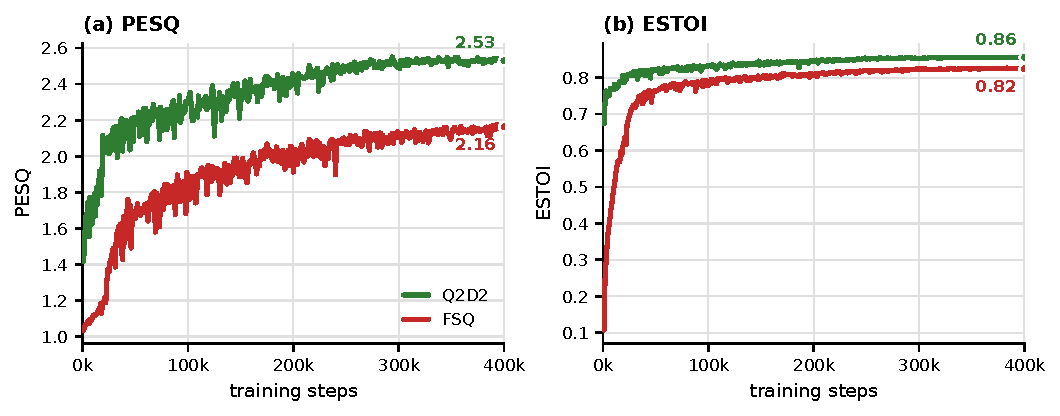
\includegraphics[width=0.86\textwidth]{figures/fsq_vs_q2d2_clean.pdf}
\caption{FSQ vs.\ Q2D2 at the main $12.5$\,Hz / cd64 operating point. Both
runs use the same Stage-1 JEPA encoder, decoder architecture, bitrate, losses
and $400$k-step schedule; the Q2D2 run additionally resumes from a partial
decoder warm-start, yielding a non-zero starting ESTOI. We therefore interpret
the curves as a matched final-operating-point comparison rather than a
strictly initialization-matched quantizer-only trial
(Table~\ref{tab:ablation}). Internal training-time eval.}
\label{fig:fsqq2d2}
\end{figure*}

\textbf{Quantizer diagnostics.} The $32$ per-pair affine transforms remain
well-conditioned (mean condition number $1.18$, determinants $0.99\pm0.002$),
i.e.\ they adapt without degenerating. The packed token vocabulary of $65{,}536$
is used at $17.0\%$ (entropy ratio $0.77$, effective vocabulary $\approx4{,}900$),
indicating the codec concentrates mass on a meaningful subset rather than
collapsing to a few codes or spreading uniformly.

\subsection{SIGReg co-design}
\label{sec:sigreg}

Whether the encoder needs SIGReg depends on how hard the quantizer is pushed.
Table~\ref{tab:sigreg} reports a matched pair at a harder operating point,
$25$\,Hz and code dimension $32$: two Q2D2 codecs identical in architecture,
quantizer and $100$k single-phase training steps, differing only in whether the
Stage~1 encoder was trained with the SIGReg regularizer
($\lambda_{\mathrm{sigreg}}{=}0.05$) or without it
($\lambda_{\mathrm{sigreg}}{=}0$). Without SIGReg the codec never leaves the
floor (ESTOI $-0.004$, PESQ $1.05$); with it the same codec trains normally to
ESTOI $0.79$, PESQ $2.24$. Fig.~\ref{fig:sigreg} shows the two training curves.
The collapse is specific to this aggressive regime: our main $12.5$\,Hz / cd64
model (Table~\ref{tab:recon}) is built on a plain EMA-target encoder with no
SIGReg and trains without issue. SIGReg is therefore best read as a co-design
tool that becomes necessary as the quantizer is pushed toward lower dimension
and higher frame rate, not a universal requirement for pairing Q2D2 with a JEPA
encoder.

\begin{table}[t]
\caption{SIGReg ablation at an aggressive $25$\,Hz / cd32 operating point.
Matched pair: identical architecture, quantizer and $100$k single-phase
training steps; only the Stage~1 encoder's SIGReg weight differs. Internal
training-time protocol.}
\label{tab:sigreg}
\centering
\begin{tabular}{lcc}
\toprule
Stage-1 encoder & PESQ & ESTOI \\
\midrule
\textbf{with SIGReg} ($\lambda_{\mathrm{sigreg}}{=}0.05$) & \textbf{2.24} & \textbf{0.793} \\
without SIGReg ($\lambda_{\mathrm{sigreg}}{=}0$) & 1.05 & $-0.004$ \\
\bottomrule
\end{tabular}
\end{table}

\subsection{Emergent cross-lingual structure}
\label{sec:crosslingual}

We extract \emph{pre-quantization} frame-level encoder features for six FLEURS
languages (English, French, German, Hindi, Japanese, Chinese), balance to
$539$ utterances per language, and measure how separable the languages are
under a fair protocol (standardize, PCA to $50$ dimensions, equalize frame
counts across models).
\textbf{All FLEURS speech is held out from codec training}: the codec is
trained only on LibriLight, and the English FLEURS subset is a corpus disjoint
from LibriLight. Every probe, $t$-SNE, NMI score and classifier accuracy in
this section is computed on speech the codec has never seen.
Table~\ref{tab:crosslingual} reports $5$-fold cross-validated classifier
accuracy; chance is $0.167$. To test whether frame-level $5$-NN probes exploit
utterance leakage, we repeated the evaluation with utterance-disjoint folds.
Scores changed negligibly: JEPA-EMA drops from $0.854$ to $0.850$, JEPA-SIGReg
from $0.793$ to $0.791$, and the cross-model ordering is unchanged.

\begin{table}[t]
\caption{Language separability of pre-quantization frame-level features on
FLEURS (6 languages, 5-fold CV, chance $=0.167$). [E]\,=\,English-only training,
[M]\,=\,multilingual. Our codec is English-only and a $1.6$\,kbps reconstruction
codec; SSL models are uncompressed representation models. Utterance-disjoint
$5$-NN gives nearly identical scores: JEPA-EMA $0.850$, JEPA-SIGReg $0.791$.}
\label{tab:crosslingual}
\centering
\begin{tabular}{llccc}
\toprule
Model & Type & LogReg & SVM & 5-NN \\
\midrule
wav2vec2-base       & SSL [E]    & 0.855 & 0.847 & \textbf{0.925} \\
\textbf{Ours (JEPA-EMA)} & \textbf{codec [E]} & 0.605 & 0.598 & \textbf{0.854} \\
Ours (JEPA-SIGReg)  & codec [E]  & 0.729 & 0.715 & 0.795 \\
XLS-R-300m          & SSL [M]    & 0.685 & 0.669 & 0.752 \\
Mimi                & codec      & 0.499 & 0.489 & 0.634 \\
mHuBERT-147         & SSL [M]    & 0.484 & 0.471 & 0.612 \\
EnCodec             & codec      & 0.405 & 0.395 & 0.605 \\
HuBERT-base         & SSL [E]    & 0.409 & 0.400 & 0.563 \\
DAC                 & codec      & 0.385 & 0.382 & 0.451 \\
\bottomrule
\end{tabular}
\end{table}

Three findings stand out. (i) Among neural codecs ours preserves cross-lingual
structure by a wide margin ($85.4\%$ vs.\ Mimi $63.4\%$, EnCodec $60.5\%$,
DAC $45.1\%$ on $5$-NN). (ii) Our English-only $1.6$\,kbps codec exceeds
multilingually-trained SSL (XLS-R $75.2\%$, mHuBERT $61.2\%$) and approaches
uncompressed English wav2vec2-base ($92.5\%$). (iii) In this comparison codec
architecture appears to dominate training-data multilinguality: multilingually
trained EnCodec and DAC carry far less language structure than our
English-only codec. We do not claim JEPA uniquely produces cross-lingual
structure (wav2vec2-base is better at it, and the phenomenon is documented in
prior SSL work); our claim is the \emph{codec} result, with the additional
point that our system is the only entry in Table~\ref{tab:crosslingual} that
pairs an SSL-style predictive objective with full audio reconstruction.

\begin{figure}[H]
\centering
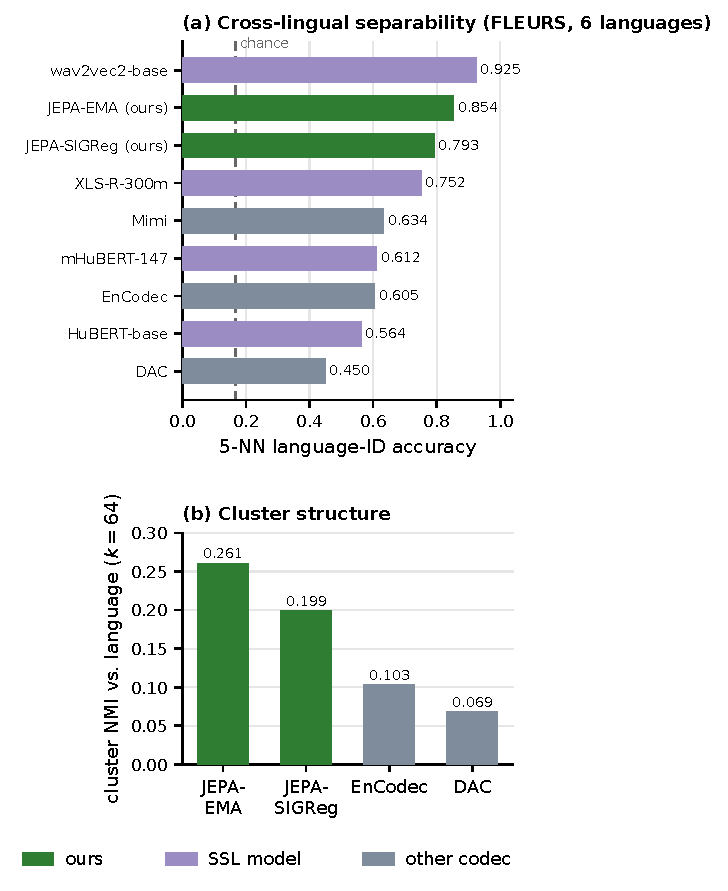
\includegraphics[width=\columnwidth]{figures/crosslingual_summary.pdf}
\caption{Cross-lingual structure on six held-out FLEURS languages (five unseen during codec training; English subset disjoint from LibriLight).
(a)~$5$-NN language-ID accuracy: our English-only $1.6$\,kbps codec exceeds
every other neural codec and every multilingually-trained SSL model we test,
approaching uncompressed English wav2vec2-base. (b)~cluster NMI against
language ($k{=}64$): our encoder forms language-correlated clusters where
EnCodec and DAC are diffuse.}
\label{fig:crosslingual}
\end{figure}

Cluster analysis (k-means, $k{=}64$) supports the same picture: our encoder has
the highest NMI against language labels among codecs ($0.26$ vs.\ EnCodec
$0.10$, DAC $0.07$) and a positive silhouette, whereas EnCodec/DAC clusters are
near-degenerate. We also repeat the analysis on \emph{speech-only frames}
(silence removed by an energy threshold), to rule out that the structure is
driven by silence regions: the ordering is preserved and our codec retains the
highest NMI ($0.236$ vs.\ EnCodec $0.091$, DAC $0.058$ at $k{=}64$).
Fig.~\ref{fig:speechtsne} shows the corresponding speech-only frame-level
$t$-SNE and the acoustic-category breakdown: the JEPA codecs visibly partition
the six languages while DAC remains diffuse, and labelling each cluster by
coarse acoustic descriptors (RMS, ZCR, spectral centroid, F0 via pYIN with
confidence masking) groups the $64$ clusters into five interpretable
categories. The encoder's language structure is thus carried by
acoustic-functional groupings rather than an opaque code.

\begin{figure}[H]
\centering
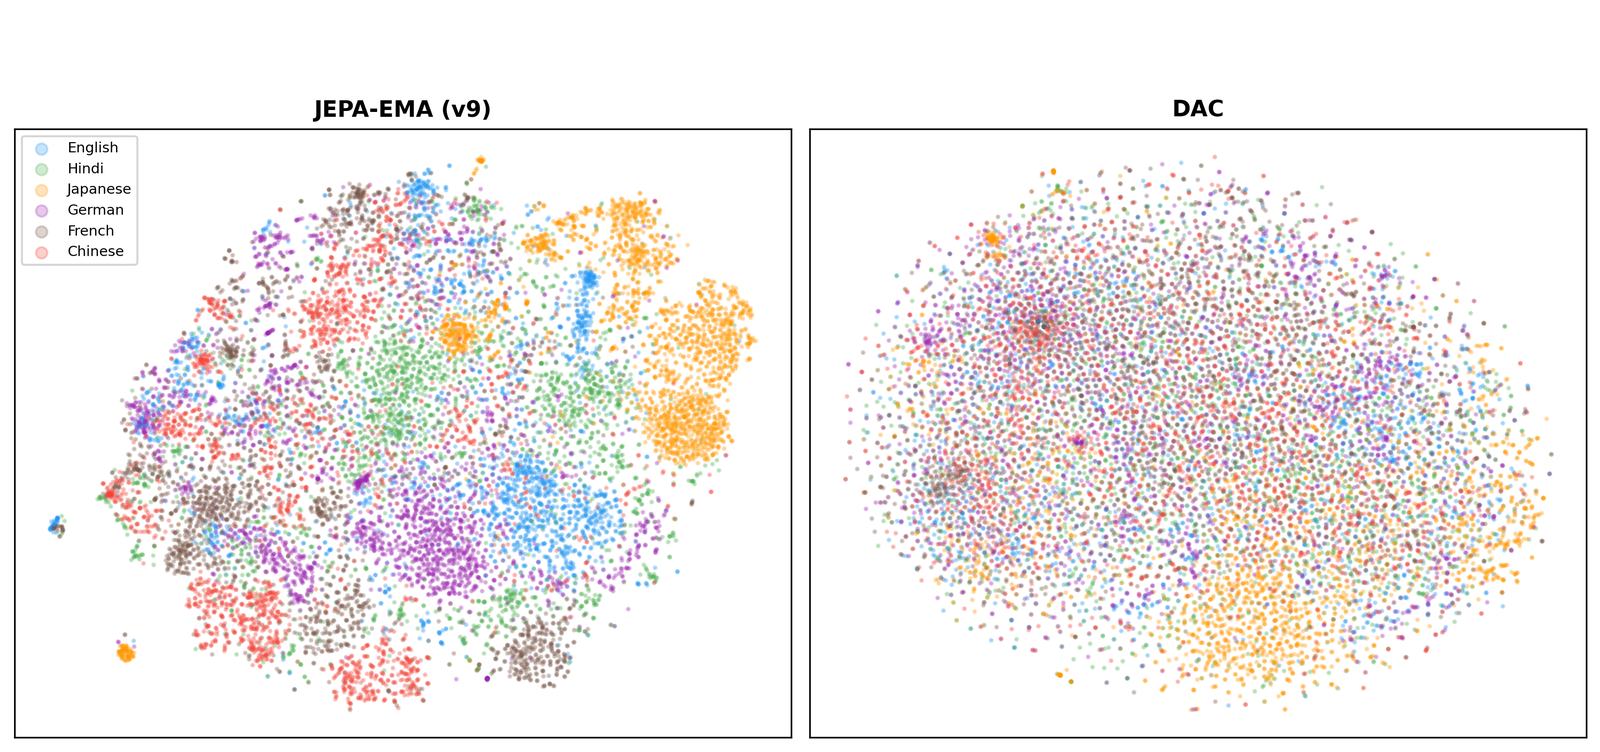
\includegraphics[width=\columnwidth]{figures/speech_only_tsne_2panel.png}
\caption{Speech-only frame-level $t$-SNE (silence removed), coloured by
language. JEPA-EMA (left): the six FLEURS languages form distinct clusters;
DAC (right): diffuse, no language structure. The $64$ JEPA clusters partition
into $15$ frication / $15$ sonorant-vowel / $14$ unvoiced-plosive / $17$ mixed
/ $3$ low-energy transition.}
\label{fig:speechtsne}
\end{figure}

\subsection{Style separation across language}

As a secondary probe on \textbf{held-out Hindi emotional speech} (the codec
has seen no Hindi during training), we classify five emotion classes
(whisper, angry, excited, neutral, sad; chance $0.20$) at utterance level:
JEPA-SIGReg reaches $63.4\%$ LogReg, JEPA-EMA $51.3\%$ $5$-NN, ahead of
EnCodec ($37.3\%$) and DAC ($30.8\%$); on the binary whisper-vs-angry case the
gap widens (JEPA-SIGReg $95.8\%$ LogReg, vs.\ Mimi $80.4\%$). Fig.~\ref{fig:emotion}
shows the utterance-level $t$-SNE: JEPA codecs cluster emotions where EnCodec
and DAC primarily separate only whisper.

\begin{figure*}[!htbp]
\centering
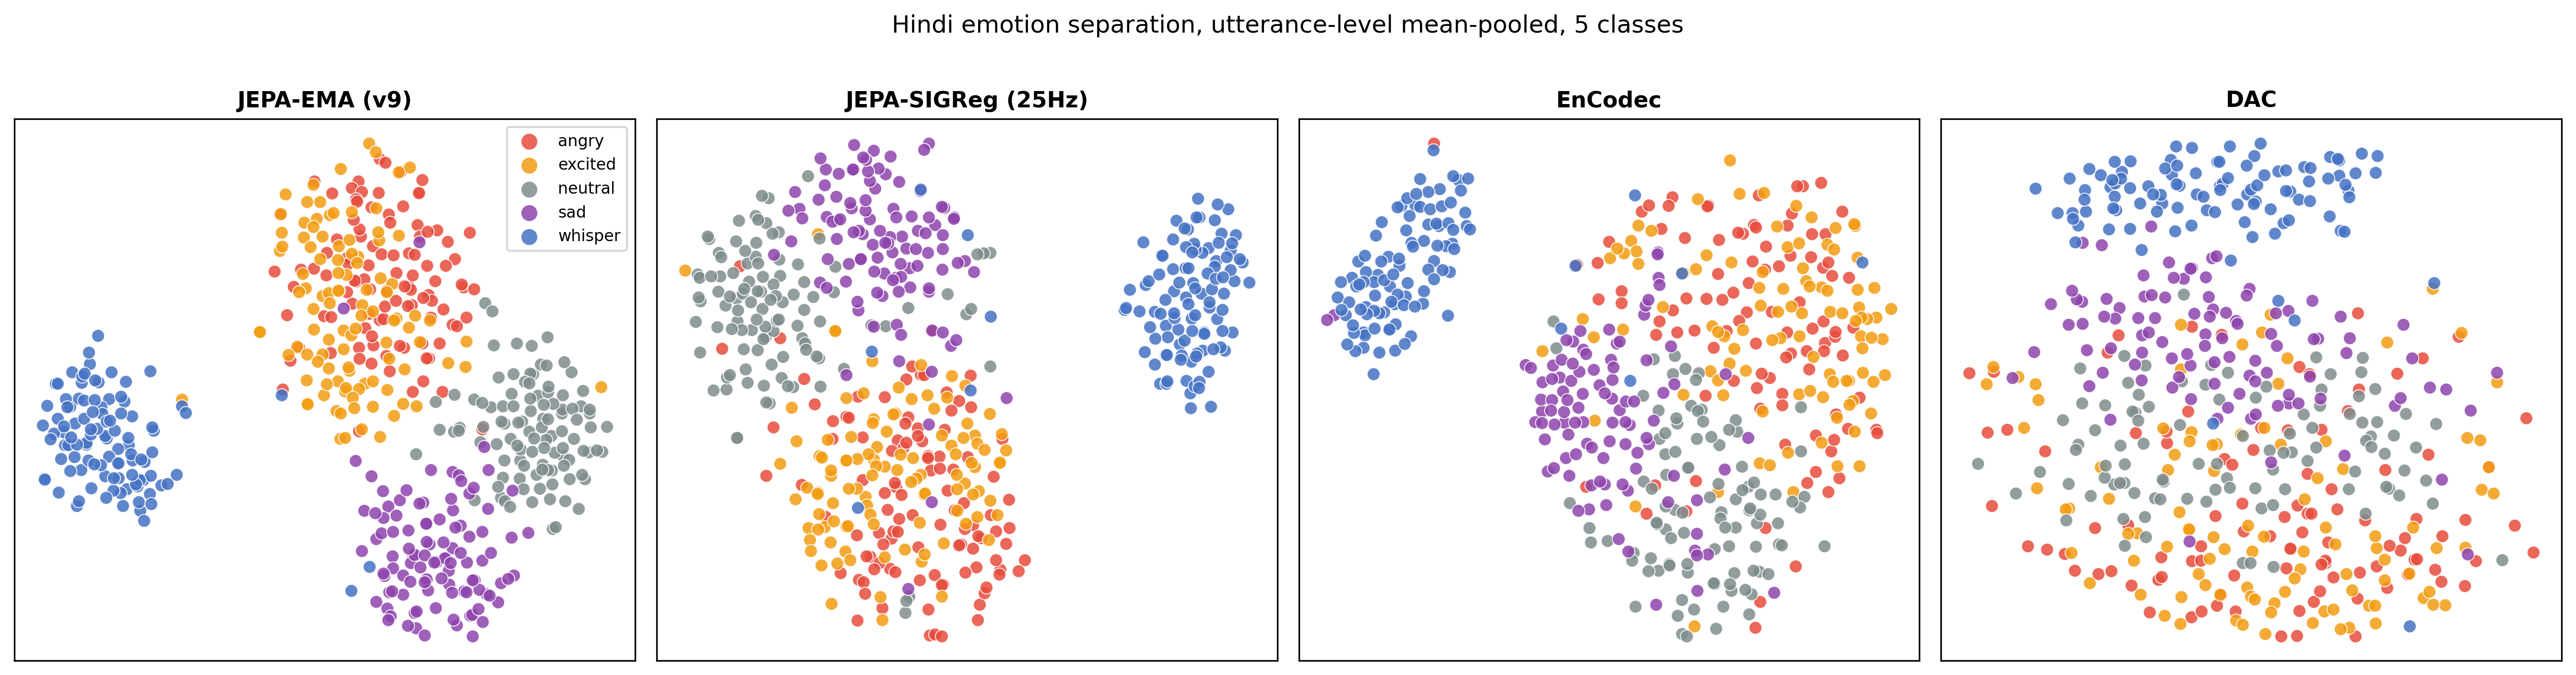
\includegraphics[width=\textwidth]{figures/emotion_tsne.png}
\caption{Five-class Hindi emotion separation, utterance-level $t$-SNE on a
held-out corpus the codec never saw during training. JEPA codecs (ours; left
two panels) form per-emotion clusters; EnCodec and DAC primarily separate
whisper from the rest. Five classes, balanced; codec trained on English
LibriLight only.}
\label{fig:emotion}
\end{figure*}

\section{Related Work}

\textbf{Neural speech codecs.} SoundStream \cite{soundstream} and EnCodec
\cite{encodec} established the RVQ-GAN paradigm; DAC \cite{dac} improved it with
better quantizer training. Recent low-bitrate codecs include Mimi
\cite{mimi}, WavTokenizer \cite{wavtokenizer}, BigCodec \cite{bigcodec} and
SpeechTokenizer \cite{speechtokenizer}. We differ in using a JEPA encoder, a
lattice quantizer, and no discriminator.

\textbf{Quantization.} FSQ \cite{fsq} removes codebook learning with
axis-aligned scalar grids; Q2D2 \cite{q2d2} generalizes this to two-dimensional
lattices with per-pair affines and was introduced as an audio codec with a
conventional encoder. Our contribution is not Q2D2 itself but pairing it with
a JEPA encoder and identifying when that pairing needs a Gaussianized source
distribution (SIGReg).

\textbf{Self-supervised speech and JEPA.} wav2vec\,2.0 \cite{wav2vec2}, HuBERT
\cite{hubert} and WavLM \cite{wavlm} learn representations that, as we and
others observe, encode language identity. JEPA \cite{ijepa,vjepa} predicts
masked latents; JEPA-as-tokenizer \cite{jepa_tokenizer} first used a JEPA
encoder for audio coding, which we extend with Q2D2, SIGReg and the
cross-lingual analysis.

\section{Limitations}
\label{sec:limits}

(1)~\textbf{English-only training.} We use $\approx5.8$k hours of English-only
LibriLight, orders of magnitude less than multilingual SSL (XLS-R $436$k\,h,
$128$ languages). This is a deliberate sample-efficiency demonstration;
multilingual scale-up is future work.
(2)~\textbf{Reconstruction trails Mimi.} On the matched protocol Mimi attains
higher ESTOI at a lower bitrate; we win PESQ but the comparison is not
bitrate-matched.
(3)~\textbf{Intelligibility.} Word error rate is $23.2\%$ at $1.6$\,kbps; the
higher-bitrate reference codec reaches $8.6\%$ under the identical protocol.
Low-frame-rate codecs have a known intelligibility ceiling, and the FSQ variant
preserves lexical content better than Q2D2 at this bitrate ($19.4\%$).
(4)~\textbf{wav2vec2-base beats us on cross-lingual separability;} our claim is
restricted to ``best among codecs'' and ``competitive with uncompressed SSL
while being a $1.6$\,kbps codec.''
(5)~\textbf{Acoustic categories are heuristic} (signal descriptors, not forced
alignment) and no bitrate-matched comparison to BigCodec / WavTokenizer /
SemantiCodec is included; only Mimi was run as a low-bitrate baseline.

\section{Conclusion}

We presented a $1.6$\,kbps JEPA speech codec built on Q2D2 lattice
quantization and trained without adversarial losses. At the main $12.5$\,Hz /
cd64 operating point, Q2D2 improves PESQ over FSQ by $+0.37$ under a matched
internal ablation protocol; separately, a $25$\,Hz / cd32 experiment shows
that SIGReg can prevent Q2D2 collapse when the bottleneck is pushed harder, a
concrete instance of distribution-quantizer co-design. On held-out FLEURS
speech, the English-trained codec's pre-quantization encoder features exhibit
stronger cross-lingual acoustic structure than every other neural-codec
baseline we test, with the structure carried by interpretable acoustic
categories. We hope the quantizer recipe and the analysis are useful beyond
this specific codec.

\FloatBarrier
{\footnotesize
\bibliographystyle{IEEEtran}
\bibliography{references}
}

\end{document}
